\chapter{数理モデル最適化}
\label{chap::math}

\hspace{1zw}本章では,オフィスビルの一室の空調設定スケジュールを最適化するため,数理モデルを用いる手段について述べる.
\section{概要}

\subsection{システム構成}
\hspace{1zw}数理モデルによる最適化システムの構成を\figref{fig::math_system}に示す.本システムは,最適化部と評価部からなる.評価部は,最適化部から空調設定温度スケジュール(解)を受け取り,数理モデルに基づいて室内快適性とエネルギー消費量を算出して最適化部に渡す.最適化部は,その結果に基づいて解を比較し,新しい解の生成を繰り返す.本システムの出力は,最適化された空調設定スケジュール集合である.

\begin{figure*}[t]
  \begin{center}
    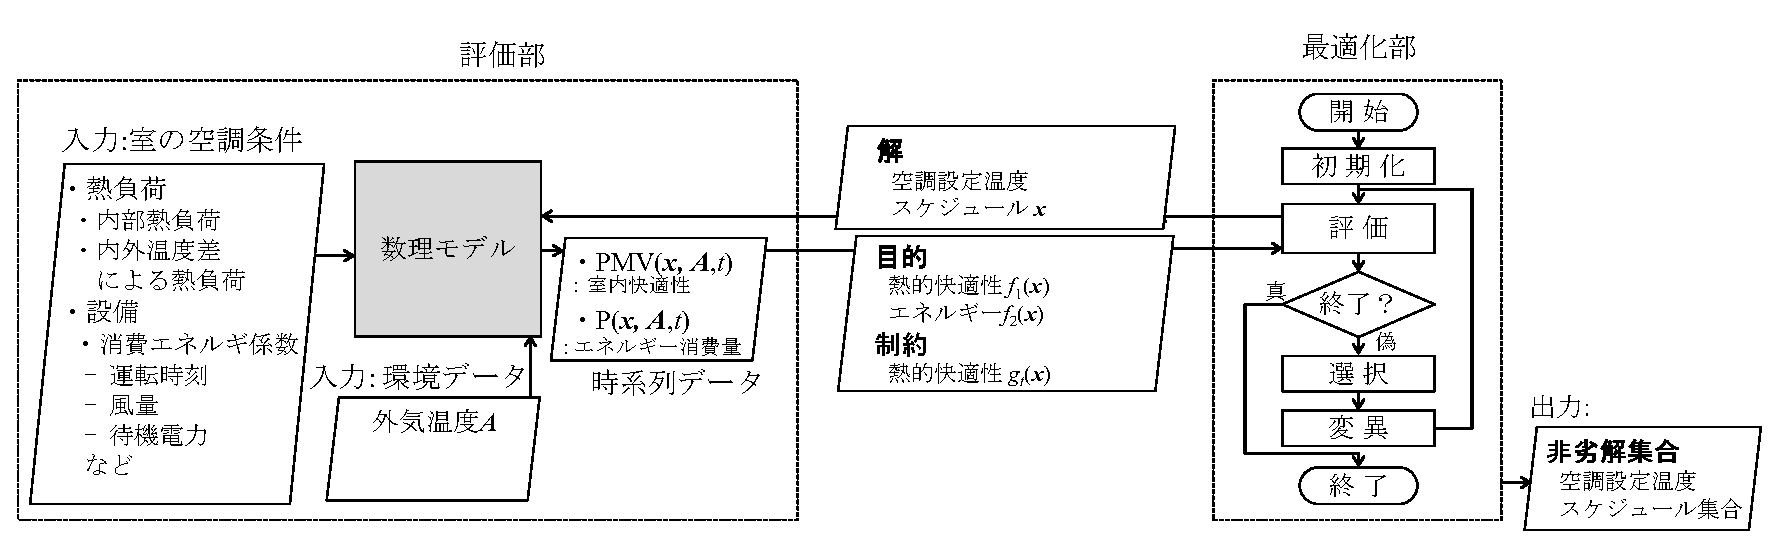
\includegraphics[width=1.1\linewidth]{fig/math_system.eps}
  \end{center}
  \vspace{-0.5cm}
  \caption{数理モデル最適化システム}
  \label{fig::math_system}
\end{figure*}


\subsection{最適化対象のオフィス}
本章では,\figref{fig::math_office_room}に示すオフィスの一室を対象にする.本空調環境は,東京都内の8階建てビルの5階に位置する窓のない部屋で,広さは37.6 [m$^2$]である.この部屋にはビル用マルチエアコンが設置されている.エアコンは,独立した室外機と冷媒系統を用い,冷暖房能力7.1 [kW]の4方向吹出口を持つ室内機を2台設置している.部屋の広さと空調機の能力を\tabref{tab::math_office_spec}に示す.

\begin{figure}[t]
  \begin{center}
    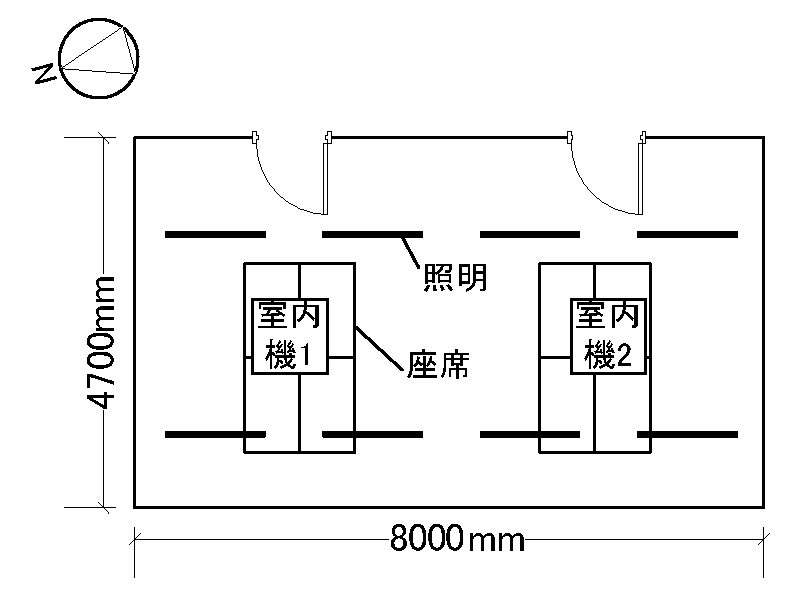
\includegraphics[width=0.6\linewidth]{fig/math_office_room.eps}
  \end{center}
  \vspace{-0.5cm}
  \caption{オフィスビルの1室}
  \label{fig::math_office_room}
\end{figure}

\begin{table}[b]
  \caption{空調環境諸元}
  \label{tab::math_office_spec}
  \centering
  \begin{tabular}{c|cccc}
    \hline
    項目           & 値               \\
    \hline    \hline
    面積[m$^2$]    & 37.6             \\
    室外機能力[kW] & 14               \\
    室内機能力[kW] & 7.1$ \times $2台 \\
    \hline
  \end{tabular}
\end{table}

\section{数理モデル最適化における解評価}
本節では,上述のオフィスの部屋に対して適用する空調設定スケジュールの評価を行うために目的関数を定義し,空調設定スケジュール最適化問題を多目的最適化問題として定式化する.

\subsection{設計変数}
従来の空調システムは,ビル管理者が,季節または月・日ごとに,これまでのエネルギー消費量の傾向と室内環境の履歴から,当日の設定温度を決定する.空調設定温度スケジュール最適化では空調の設定温度を分割時間間隔$T_s$毎に変更することとし,1日の設定温度スケジュール$t_{set}(\vec{x},t) (t \in \mathcal{T}_{set})$を最適化する.本章では,$T_s=0.5$[hour]とし設定可能時刻集合を$\mathcal{T}_{set}=\{8:00, 9:30,\dots, 22:00\}$とする.
設定温度スケジュール$t_{set}(\vec{x},t)$を設計変数ベクトル$\vec{x}$で表すためには,以下のように,設計変数ベクトルの各要素$x_t$を設定可能時刻$t$における設定温度$t_{set}(\vec{x},t)$とする方法が考えられる.
\begin{equation}
  t_{set}(\vec{x},t) = x_t ~~~~~~~(t \in \mathcal{T}_{set})
  \label{eq::math_variable}
\end{equation}

しかしながら,この手法では後述の制約条件\Eqref{eq::math_constraint_tset_diff}を満たさないスケジュールが多く探索空間が膨大となり,良好な解の探索に時間がかかる.そこで,本研究では以下の通り,設計変数ベクトルの1つ目の要素は空調設定温度スケジュールの初期温度,設計変数ベクトルの2つ目以降の要素は空調設定温度スケジュールの前の時刻との差を示すものとする.

\begin{align}
  t_{set}(\vec{x},t) & =
  \begin{cases}
    x_t ~~~~~~~~~~~~~~                          & (t=8:00)                 \\
    t_{set}(\vec{x},t-T_s) + x_t ~~~~~~~~~~~~~~ & (t=8:30, 9:00,...,22:00) \\
  \end{cases}
  \label{eq::math_variable_diff}
\end{align}

\subsection{第一目的関数}
第一目的は,室内快適性の向上である.オフィスワーカーの快適性の評価が可能な快適性指標には様々なものがあるが,ここでは,PMV (Predicted Mean Vote)を用いる.PMVは,国際標準化機構(International Standardization Organization, ISO)によって標準化された室内の平均的な温冷感の指標である\cite{ISO05}.PMVは,室内の平均的な温度,湿度,風速,平均放射温度の4つの環境計測値およびオフィスワーカーの代謝量,着衣量の2つの人に依存する物理量から,温冷感を$-3$(寒い)から$+3$(暑い)までの7段階で算出する.PMV=0が最も快適な環境である.PMVの絶対値が大きいほど,不快な環境になる.第一目的関数を次式で定義する.

\begin{equation}
  \mbox{Minimize} \quad f_1(\vec{x},\mathcal{A}) = \frac{1}{|\mathcal{T}_1|} \sum_{t\in \mathcal{T}_1} | PMV(\vec{x},\mathcal{A},t) |
  \label{eq::math_objective1}
\end{equation}

ここで,$\mathcal{T}_1$は室内快適性を計測する時刻集合であり,設計変数ベクトルと同様30分間隔で$\mathcal{T}_1=\{7:00, 7:30,\dots, 21:30, 22:00\}$とする.
$PMV(\vec{x},\mathcal{A},t)$は,時刻$t$におけるPMVであり,外気温の影響を受けるため,30分ごとの外気温集合$\mathcal{A}=\{a_{00:00},a_{00:30},\dotsc,a_{23:30},a_{24:00}\}$を入力する.

本章では,$PMV(\vec{x},\mathcal{A},t)$の算出にISOが定義する以下の数理モデルを採用した.
\begin{align}
   & PMV(\vec{x},\mathcal{A},t) = (0.303\mathrm{e}^{-0.036M}+0.028)\cdot \nonumber \\
   & ~~~~~~~~~ H(T_a(\vec{x},t), R_h, V_a(t), T_r(\vec{x},t), M, I_{cl})
  \label{eq::math_pmv}
\end{align}
ここで,$H(T_a, R_h, V_a, T_r, M, I_{cl})$は人体の発熱量を示す関数である.また,$T_a(\vec{x},t)$は温度[$^o$C],$R_h$は湿度$[\%]$, $V_a(t)$は風速[m/s],$T_r(\vec{x},t)$は平均放射温度[$^o$C],$M$は代謝量[met],$I_{cl}$は着衣量[clo]である.本来,環境計測値は,空調設定および外気温$\mathcal{A}$や外気導入量等によって変動し,代謝量・着衣量は人によって異なるが,ここでは単純化のために,下記の式のように,温度および平均放射温度が空調設定スケジュール$\vec{x}$のみによって変動するものとし,他の湿度,風速,着衣量,代謝量は固定値か季節で一定の値とした.
\begin{align}
  T_a(\vec{x},t) & =
  \begin{cases}
    t_{set}(\vec{x},t) + 1.0 (夏季) & \\
    t_{set}(\vec{x},t) - 1.0 (冬季) & \\
  \end{cases}
  \label{eq::math_temperature}
\end{align}
\begin{align}
  T_r(\vec{x},t) & =
  \begin{cases}
    T_a(\vec{x}, t) + 0.2 (夏季) & \\
    T_a(\vec{x}, t) - 0.2 (冬季) & \\
  \end{cases}
  \label{eq::math_radiation}
\end{align}
\begin{align}
  R_h & =
  \begin{cases}
    55 (夏季) & \\
    45 (冬季) & \\
  \end{cases}
  \label{eq::math_humidity}
\end{align}
\begin{align}
  V_a & =V_{in}-1.0
  \label{eq::math_airvolume}
\end{align}
\begin{align}
  I_{cl} & =
  \begin{cases}
    0.6 (夏季) & \\
    0.8 (冬季) & \\
  \end{cases}
  \label{eq::math_cloth}
\end{align}
\begin{align}
  M & =1.1
  \label{eq::math_metabolic}
\end{align}
ただし,$V_{in}$は空調機の風量設定値[m$^3$/min]である.

\subsection{第二目的関数}
第二目的は,エネルギー消費量の最小化である.設計変数$\vec{x}$のエネルギー消費量に関する目的関数を次式で表す.
\begin{equation}
  \mbox{Minimize} \quad f_2(\vec{x},\mathcal{A}) = \sum_{t\in \mathcal{T}_2} P(\vec{x},\mathcal{A},t)
  \label{eq::math_objective2}
\end{equation}
ここで,$\mathcal{T}_2$はエネルギー消費量を計測する時刻集合であり,$\mathcal{T}_2=\{0:00, 0:30,\dots, 24:00\}$とする.$P(\vec{x},\mathcal{A},t)$は,時刻$t$のエネルギー消費量[W]であり,外気温集合$\mathcal{A}$の影響を受ける.

本章では,エネルギー消費量$P(\vec{x},\mathcal{A},t)$の算出に数理モデルを用いる.
\figref{fig::math_office_room}の空調システムのエネルギー消費量$P(\vec{x},\mathcal{A},t)$を,空調機にかかる熱負荷を用いて算出する\cite{Kuki12}.熱負荷は,空調機が部屋の空間に対して供給/除去する熱量である.熱負荷は,本来,建物の熱貫流や日射,換気,蓄熱,空気の移動などを考慮して算出するが,ここでは,簡易的に室内に発生する内部熱負荷と,室外との間で発生する外部熱負荷を用いて次式で算出する.
\begin{align}
  Q_{in}(t)                      & = Q_{people}(t) + Q_{light}(t) + Q_{oa}(t)
  \label{eq::math_heatload_in}                                                \\
  Q_{out}(\vec{x},\mathcal{A},t) & = (a_t - t_{set}(\vec{x},t)) Q_{temp}
  \label{eq::math_heatload_out}
\end{align}
\vspace{-0.8cm}
\begin{align}
  Q(\vec{x},\mathcal{A},t) & =
  \begin{cases}
    Q_{out}(\vec{x},\mathcal{A},t) + Q_{in}(t)~(冷房時) & \\
    Q_{out}(\vec{x},\mathcal{A},t) - Q_{in}(t)~(暖房時) & \\
  \end{cases}
  \label{eq::math_heatload}
\end{align}
ここで,$Q(\vec{x},\mathcal{A},t) $は総熱負荷,$Q_{people}(t)$は人体の熱負荷[W],$Q_{light}(t)$は照明の熱負荷[W],$Q_{oa}$は機器熱負荷[W],$Q_{temp}$は室内外温度差による熱負荷基準値[W/$^o$C]である.
空調システムが上述の熱負荷を処理するために必要とするエネルギー量$P$は,外気温度や空調機の動作条件によって変動するが,ここでは熱負荷に比例するものと仮定し次式で算出する.
\begin{align}
  P(\vec{x},\mathcal{A},t) & = P_zQ(\vec{x},\mathcal{A},t)+P_{fin}V_{fin}+P_{out}
  \label{eq::math_energy}
\end{align}
ここで,$P_z$は熱負荷とエネルギー消費量との比例係数,$P_{fin}$は室内機の風量$V_{fin}$と室内機ファンのエネルギー消費量の比例係数[$W \cdot$ min / m$^3$],$P_{out}$は室外機の待機電力[W]である.

\subsection{制約条件}
\subsubsection{快適性に関する制約}
快適性に関する制約条件を設ける.ISOでは,室内の不快な環境を避けるため,不満足者率が10\%以下となるようPMV値を$-0.5$から$+0.5$の範囲内に保つことを推奨している.そこで,次式で示すPMV値の絶対値の上限値を設定する.
\begin{equation}
  \mbox{Subject\ to} ~~~g_t(\vec{x})=|PMV(\vec{x},\mathcal{A}, t) |  \leq 0.5\quad(t \in \mathcal{T}_1)
  \label{eq::math_constraint_pmv}
\end{equation}
全ての時刻$t$に対して上記の制約条件を満たす解を実行可能解,ひとつでも満たさない時刻がある解を実行不可能解とする.制約総違反量$v(\vec{x})$を次式で表す.
\begin{equation}
  v(\vec{x}) = \sum_{t\in \mathcal{T}_1}  \max_{}{\{0,~g_t(\vec{x})-0.5\}}
  \label{eq::math_constraint_violation_pmv}
\end{equation}

\subsubsection{空調設定温度に関する制約}
空調設定温度は,設定できる値と範囲が空調機の機種によって制限される.本章では,設定可能な値は最大値・最小値の範囲内とする.また,設定温度は0.5[$^o$C]刻みで設定できるものとする.さらに,設定温度の大きく変更することによる突発的なエネルギー消費の増加を避けるため,隣接した時間帯では設定温度の変更量を$\pm1$[$^o$C]以内に制限する.これらを制約条件とし,以下の\Eqref{eq::math_constraint_tset_minmax}~\eqref{eq::math_constraint_tset_diff}で表す.
\begin{eqnarray}
  T_{min} \leq t_{set}(\vec{x},t) & \leq T_{max}
  \label{eq::math_constraint_tset_minmax} \\
  2 t_{set}(\vec{x},t) & \in \bf{Z}
  \label{eq::math_constraint_tset_int} \\
  |t_{set}(\vec{x},t) - t_{set}(\vec{x},t-T_{s})| & \leq 1
  \label{eq::math_constraint_tset_diff}
\end{eqnarray}
ここで,$T_{min}$,$T_{max}$はそれぞれ設定温度として設定可能な最小値,最大値である.また,$\bf{Z}$は整数の全体からなる集合である.

これらの設定温度に関する制約のうち\Eqref{eq::math_constraint_tset_int}および\Eqref{eq::math_constraint_tset_diff}は,設計変数が実数で設定された場合に,制約を満たすことが難しく,実行可能範囲が狭くなってしまい進化計算による探索を遅らせる原因になる.そこで,以下2つによりこれらの制約の範囲が解探索空間となるような工夫を行う.
\begin{enumerate}
  \item 設計変数ベクトルの各要素$x_t$が設定温度スケジュールの各時刻の設定温度$t_{set}(\vec{x},t)$を直接表す\Eqref{eq::math_variable}の形態ではなく,\Eqref{eq::math_variable_diff}のように設計変数ベクトルの1つ目の要素は空調設定温度スケジュールの初期温度,設計変数ベクトルの2つ目以降の要素は空調設定温度スケジュールの次の時刻との差を示すものとする.差を\Eqref{eq::math_constraint_tset_diff}を満たすよう$\pm$1[$^o$C]とすることで,制約範囲内の解のみを探索することにする.
  \item 設計変数から得られる空調設定スケジュールは実数の値であるが,これを最も近い\Eqref{eq::math_constraint_tset_int}を満たす値に丸めることとする.
\end{enumerate}

\section{実験内容}\label{sec::math_setting}
空調設定スケジュール最適化のために,前節で定義した空調設定スケジュール最適化問題に対して\subsecref{subsec::OMOPSO}で述べたOMOPSOアルゴリズムを適用して,パレート解集合を探索する.OMOPSOを採用した理由として以下が挙げられる.

\begin{itemize}
  \item OMOPSOはいくつかのベンチマークで,多目的最適化手法として代表的なNSGA-IIより良好な性能を持つこと\cite{Godinez10}
  \item 空調設定スケジュール最適化問題に類似した照明制御の問題において良好な性能を持つこと\cite{Ohta13}
  \item パラメータが乱数化されていて細かな調整が不要であること
  \item 良好な解を無制限に保存する仕組み(アーカイブ)を持ち,他の固定サイズアーカイブを持つ手法と比べてより多数の有用な解を意思決定者に提示できること
\end{itemize}

空調環境の条件は,冬季の晴れの日を想定して\tabref{tab::math_param_condition}のように定める.外気温$T_{out}$及び人体熱負荷$Q_{people}$・照明熱負荷$Q_{light}$・機器熱負荷$Q_{oa}$は時間帯によって変動する.外気温の1日の推移を\figref{fig::math_outside_temp}に,人体熱負荷$Q_{people}$,照明熱負荷$Q_{light}$,機器熱負荷$Q_{oa}$を合わせた内部熱負荷$Q_{in}$の1日の推移を\figref{fig::math_internal_heatload}に示す.対象オフィスでは12時~13時の間は昼休みであり,オフィスの在室者が減り内部熱負荷が減少する.そのため,12時~13時の時間帯は\Eqref{eq::math_constraint_pmv}のPMV値に関する制約を満たさなくても良いものとする.

\begin{figure}[ht]
  \begin{center}
    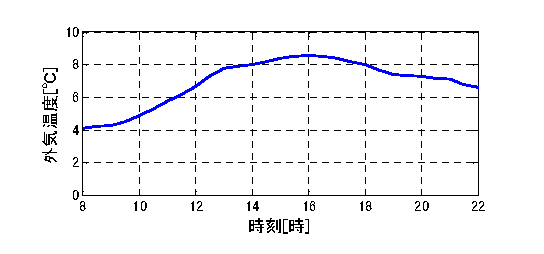
\includegraphics[width=85mm]{fig/math_outside_temp.eps}
  \end{center}
  \caption{外気温$T_{out}$の時間推移}
  \label{fig::math_outside_temp}
\end{figure}
\begin{figure}[ht]
  \begin{center}
    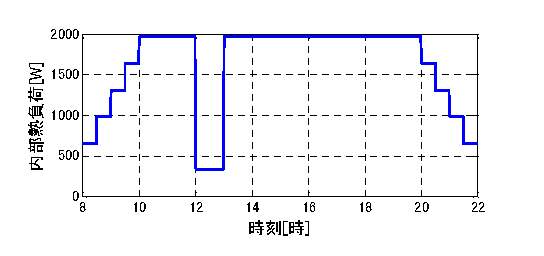
\includegraphics[width=85mm]{fig/math_internal_heatload.eps}
  \end{center}
  \caption{内部熱負荷$Q_{in}$の時間推移}
  \label{fig::math_internal_heatload}
\end{figure}

\begin{table}[htbp]
  {\small
    \begin{center}
      \caption{空調環境条件}
      \begin{tabular}{c|cccc}
        \hline
        項目                                      & 値                                           \\
        \hline    \hline
        外気温度$T_{out}$[$^o$C]                   & \figref{fig::math_outside_temp}に示す        \\
        人体熱負荷$Q_{people}$[kW]                & 3つを合計した                                \\
        照明熱負荷$Q_{light}$[kW]                 & 内部熱負荷$Q_{in}$                           \\
        機器熱負荷$Q_{oa}$[kW]                    & を\figref{fig::math_internal_heatload}に示す \\
        温度差による熱負荷基準値$Q_{temp}$[W/$^o$C] & 400                                          \\
        熱負荷-エネルギー消費量比例係数$P_z$[-]   & 0.25                                         \\
        風量-エネルギー消費量比例係数$P_{fin}$[-] & 10                                           \\
        室外機待機電力$P_{out}$[W]                & 50                                           \\
        設定温度最小値$T_{min}$[$^o$C]             & 17                                           \\
        設定温度最大値$T_{max}$[$^o$C]              & 28                                           \\
        室内機吹出風量$V_{in}$[$m^3$/$min$]           & 12                                           \\
        運転開始時刻$T_{start}$                   & 08:00                                        \\
        運転終了時刻$T_{end}$                     & 22:00                                        \\
        分割時間間隔$T_s$[hour]                   & 0.5                                          \\
        時間分割数$N_t$                           & 29                                           \\
        \hline
      \end{tabular}
      \label{tab::math_param_condition}
    \end{center}
  }
\end{table}

OMOPSOアルゴリズムのパラメータは\tabref{tab::math_param_algo}のように定める.ここで,重み$w, c_1, c_2$は文献\cite{Sierra05}の推奨値を用いた.また,$\epsilon$優越する範囲を調整する係数$\epsilon$は,値が探索結果に大きく影響する.そこで,本問題に適切な$\epsilon$の値を検討するため,$\epsilon=0, 0.0075, 0.05$と変更して複数回探索を試行した.
本章では,数理モデルおよびOMOPSOアルゴリズムをプログラミング言語Javaで実装した.計算機環境には,一般的なビル管理システムの計算能力を想定して,Windows 7 (64ビット),Intel Core i7-2600S (2.8GHz)およびRAM 8GBのPCを用いた.

\begin{table}[t]
  {\small
    \begin{center}
      \caption{OMOPSOのパラメータ}
      \label{tab::math_param_algo}
      \begin{tabular}{c|cccc}
        \hline
        パラメータ                             & 方法 / 値              \\
        \hline \hline
        ベース粒子群サイズ $N^{\mathcal{P}}$   & 100                    \\
        リーダー粒子群サイズ $N^{\mathcal{L}}$ & 100                    \\
        アーカイブ粒子群サイズ                 & 制限なし               \\
        総世代数 $g_{max}$                     & 10000                  \\
        変数帳 $n$                             & 29                     \\
        突然変異率 $p_m$                       & $1/n$                  \\
        重み $w$                               & [$0.1, 0.5$)の一様乱数 \\
        重み $c_1, c_2$                        & [$1.5, 2.0$)の一様乱数 \\
        非一様突然変異の係数 $b$               & 5 \cite{Esquivel03}    \\
        $\epsilon$優越の係数$\epsilon$         & 0, 0.0075, 0.05        \\
        \hline
      \end{tabular}
    \end{center}
  }
\end{table}

\section{実験結果と考察}
\subsection{実験結果}

数理モデル最適化によって得られた空調設定スケジュールの集合を\figref{fig::math_result_pareto_eps}に$\epsilon$の値ごとに青点で示す.
それぞれの図について,横軸が室内快適性$f_1$, 縦軸がエネルギー消費量$f_2$であり,どちらも小さいほど良好なスケジュールであることを示す.数理モデル最適化によって,$\epsilon=0$では76個,$\epsilon=0.0075$では56個,$\epsilon=0.05$では29個のスケジュールが獲得できた.数理モデル最適化によって得られたスケジュール集合は,室内快適性とエネルギー消費量のトレードオフを示すことがわかる.また,スケジュール集合は制約\Eqref{eq::math_constraint_pmv}を満たす平均$|$PMV$|$の範囲0~0.5のうち広い範囲の解を含んでいる.ただし,制約範囲の境界付近である$|$PMV$|\leq 0.1$と$|$PMV$|\geq 0.4$ の範囲では獲得された解の数が少ない.さらに,$\epsilon$の値が大きくなるごとに境界付近で良い解を探索できなくなり,解の分布が均等でなくなっている.

\begin{figure*}[htbp]
  \begin{center}
    \begin{minipage}{0.6\textwidth}
      \begin{center}
        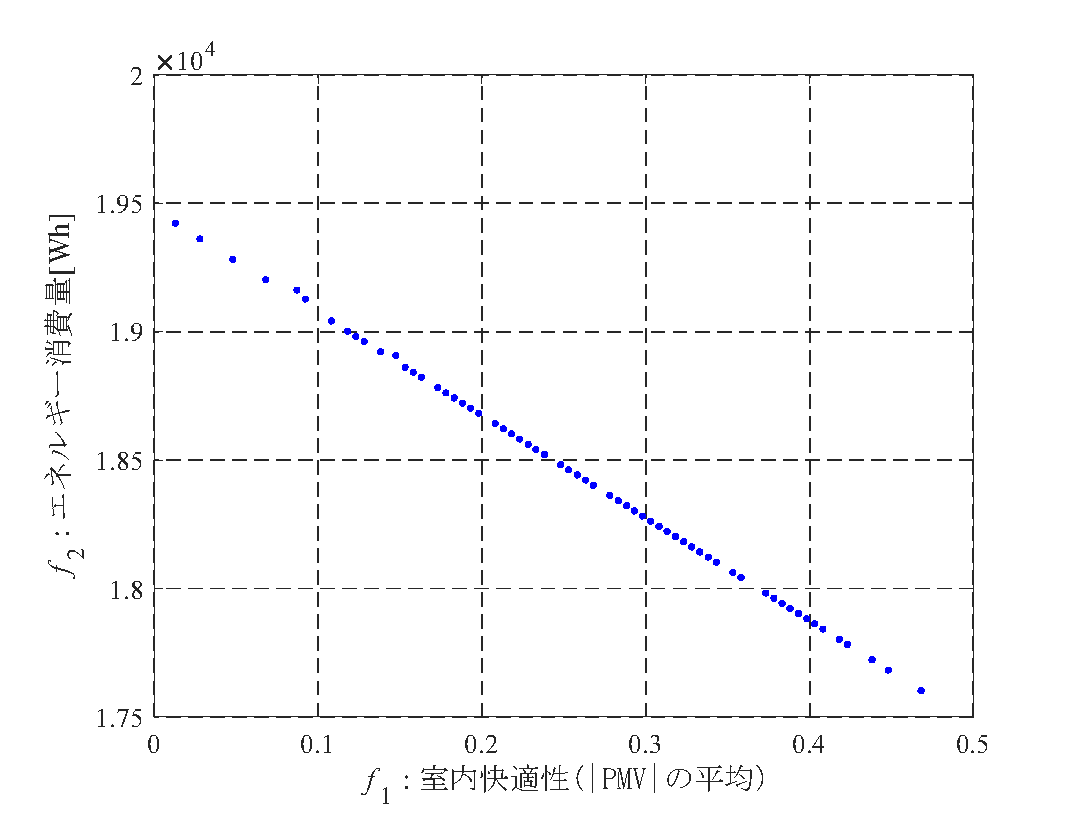
\includegraphics[width=1.0\textwidth,keepaspectratio=true]{fig/math_result_pareto_eps1.eps}\\\vspace{-0.3cm}{{(a) $\epsilon=0$}}
      \end{center}
    \end{minipage}
    \begin{minipage}{0.6\textwidth}
      \begin{center}
        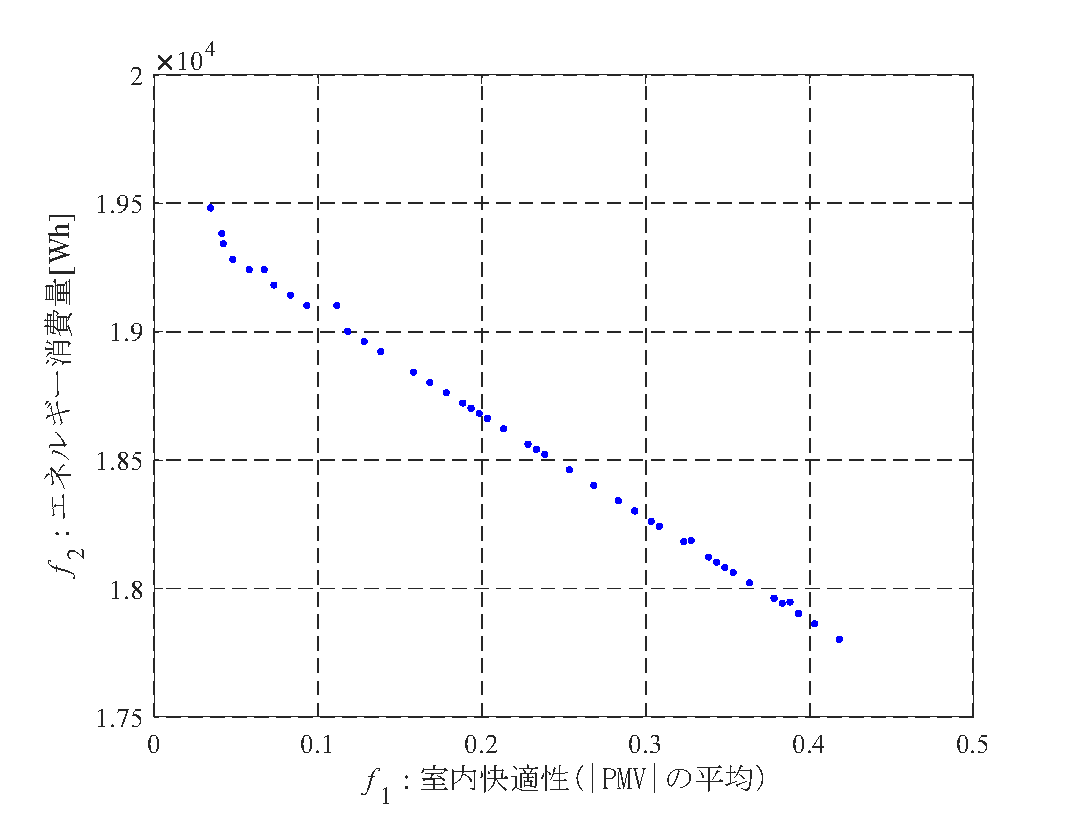
\includegraphics[width=1.0\textwidth,keepaspectratio=true]{fig/math_result_pareto_eps2.eps}\\\vspace{-0.3cm}{{(b) $\epsilon=0.0075$}}
      \end{center}
    \end{minipage}
    \begin{minipage}{0.6\textwidth}
      \begin{center}
        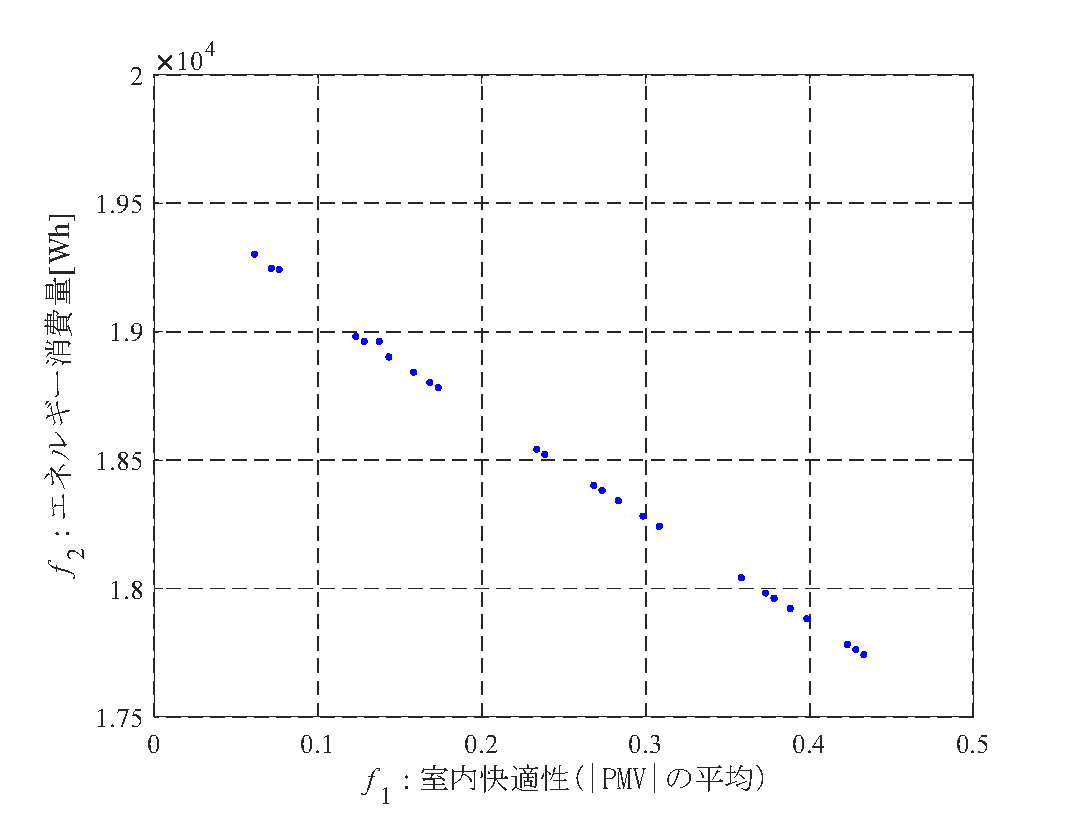
\includegraphics[width=1.0\textwidth,keepaspectratio=true]{fig/math_result_pareto_eps3.eps}\\\vspace{-0.3cm}{{(c) $\epsilon=0.05$}}
      \end{center}
    \end{minipage}
  \end{center}
  \vspace{2mm}
  \caption{$\epsilon$を変更した場合の数理モデル最適化の結果}
  \label{fig::math_result_pareto_eps}
\end{figure*}

\begin{comment}
最も広い範囲を均等に探索できた$\epsilon=0$のパレート解に対し,比較のために従来法である設定温度を終日一定値に設定した解を同一目的関数空間上に赤のアスタリスクで図示したものを\figref{fig::math_result_pareto}に示す.数理モデル最適化は,設定温度を一定にする従来法のスケジュールをパレート支配するスケジュールを獲得しており,良好なスケジュールが得られたといえる.

\begin{figure}[htbp]
  \begin{center}
    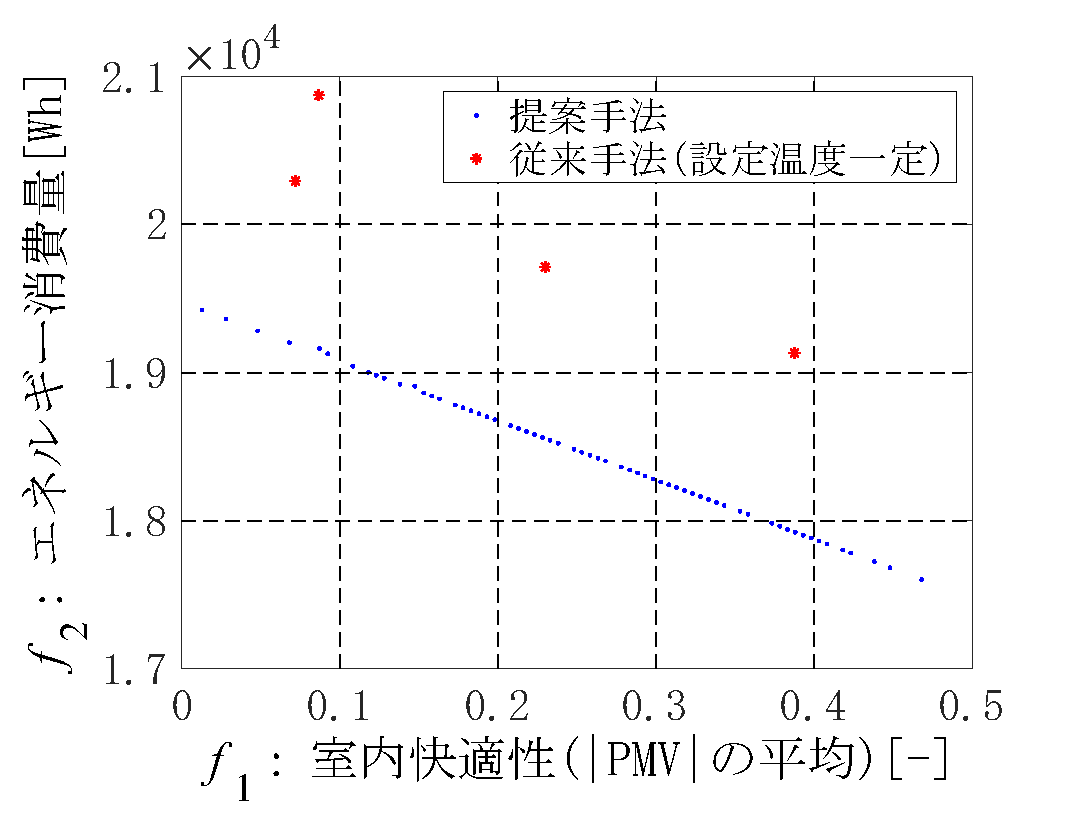
\includegraphics[width=0.7\linewidth]{fig/math_result_pareto.eps}
  \end{center}
  \caption{数理モデル最適化による解集合と設定温度一定解の比較}
  \label{fig::math_result_pareto}
\end{figure}
\end{comment}

最も広い範囲を均等に探索できた$\epsilon=0$の探索で得られたスケジュール集合のうち例として,室内快適性の目的関数値が最も小さい快適な解($f_1=0.0279$),最も値の大きい不快な解($f_1=0.463$),中間の解($f_1=0.233$)の設定温度スケジュールの例と,そのスケジュールで運転した際の快適性・エネルギー消費量の推移を\figref{fig::math_result_schedule}に示す.昼の時間帯を除き,すべての時間帯で\Eqref{eq::math_constraint_pmv}を満たすよう制御できていることがわかる.

\begin{figure}[htbp]
  \centering
  \subfigure{
    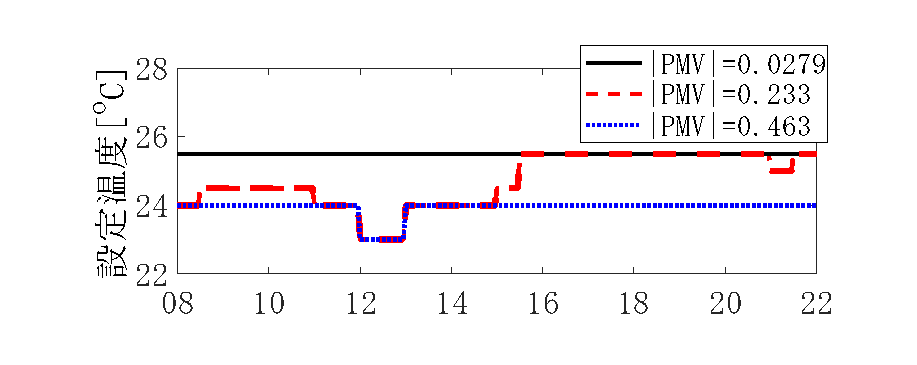
\includegraphics[width=0.6\textwidth,keepaspectratio=true]{fig/math_result_schedule_settemp.eps}
    \label{fig::math_result_schedule_settemp}
  }
  \subfigure{
    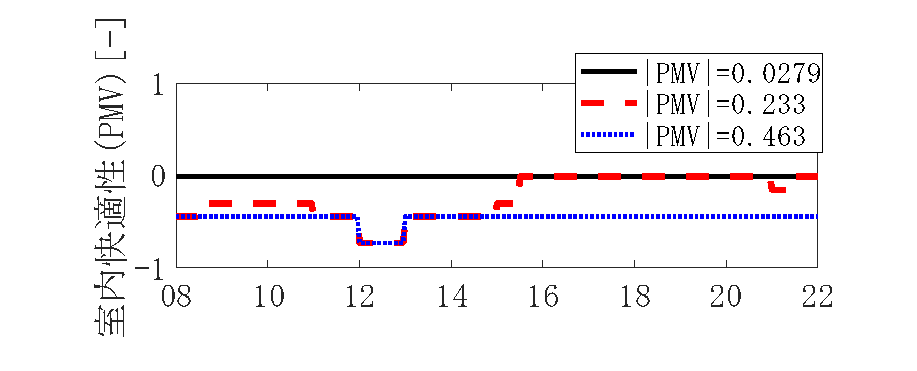
\includegraphics[width=0.6\textwidth,keepaspectratio=true]{fig/math_result_schedule_pmv.eps}
    \label{fig::math_result_schedule_pmv}
  }
  \subfigure{
    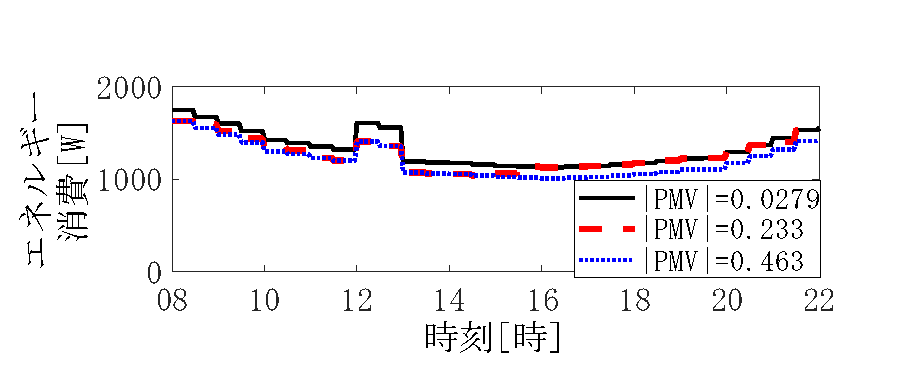
\includegraphics[width=0.6\textwidth,keepaspectratio=true]{fig/math_result_schedule_power.eps}
    \label{fig::math_result_schedule_power}
  }
  \caption{数理モデル最適化で獲得された空調設定スケジュール,室内快適性,エネルギー消費量の例}
  \label{fig::math_result_schedule}
\end{figure}
獲得された設定温度スケジュールが最も多様であった$|PMV| \approx 0.25$付近の解10個の設定温度スケジュールを確認する.それぞれの設定温度スケジュールを\figref{fig::math_result_schedule_settemp10}に示す.全体的な傾向として,どの解も15:30~17:00の時間帯は25$^o$C以上の設定温度であることがわかる.午前中は温度が低く午後に温度が高くなる解が多いが,(b)(h)のように午前中を午後よりも高い設定温度とする解や,(i)のように一日を通して設定温度がほぼ一定である解もある.また,多くの解は昼の時間帯は制約\Eqref{eq::math_constraint_pmv}を考慮せずともよくなるため設定温度が他の時間帯に対し1$^o$C程度低くなっているが,(i)の解については温度が低くなっていない.

\begin{figure*}[htbp]
  \begin{center}
    \begin{minipage}{0.4\textwidth}
      \begin{center}
        \includegraphics[width=1.0\textwidth,keepaspectratio=true]{fig/math_result_schedule_settemp_a.eps}\\\vspace{0.3cm}{{(a) $|PMV|=0.223$}}
      \end{center}
    \end{minipage}
    \begin{minipage}{0.4\textwidth}
      \begin{center}
        \includegraphics[width=1.0\textwidth,keepaspectratio=true]{fig/math_result_schedule_settemp_b.eps}\\\vspace{0.3cm}{{(b) $|PMV|=0.228$}}
      \end{center}
    \end{minipage}
    \begin{minipage}{0.4\textwidth}
      \begin{center}
        \includegraphics[width=1.0\textwidth,keepaspectratio=true]{fig/math_result_schedule_settemp_c.eps}\\\vspace{0.3cm}{{(c) $|PMV|=0.233$}}
      \end{center}
    \end{minipage}
    \begin{minipage}{0.4\textwidth}
      \begin{center}
        \includegraphics[width=1.0\textwidth,keepaspectratio=true]{fig/math_result_schedule_settemp_d.eps}\\\vspace{0.3cm}{{(d) $|PMV|=0.238$}}
      \end{center}
    \end{minipage}
    \begin{minipage}{0.4\textwidth}
      \begin{center}
        \includegraphics[width=1.0\textwidth,keepaspectratio=true]{fig/math_result_schedule_settemp_e.eps}\\\vspace{0.3cm}{{(e) $|PMV|=0.248$}}
      \end{center}
    \end{minipage}
    \begin{minipage}{0.4\textwidth}
      \begin{center}
        \includegraphics[width=1.0\textwidth,keepaspectratio=true]{fig/math_result_schedule_settemp_f.eps}\\\vspace{0.3cm}{{(f) $|PMV|=0.253$}}
      \end{center}
    \end{minipage}
    \begin{minipage}{0.4\textwidth}
      \begin{center}
        \includegraphics[width=1.0\textwidth,keepaspectratio=true]{fig/math_result_schedule_settemp_g.eps}\\\vspace{0.3cm}{{(g) $|PMV|=0.258$}}
      \end{center}
    \end{minipage}
    \begin{minipage}{0.4\textwidth}
      \begin{center}
        \includegraphics[width=1.0\textwidth,keepaspectratio=true]{fig/math_result_schedule_settemp_h.eps}\\\vspace{0.3cm}{{(h) $|PMV|=0.263$}}
      \end{center}
    \end{minipage}
    \begin{minipage}{0.4\textwidth}
      \begin{center}
        \includegraphics[width=1.0\textwidth,keepaspectratio=true]{fig/math_result_schedule_settemp_i.eps}\\\vspace{0.3cm}{{(i) $|PMV|=0.267$}}
      \end{center}
    \end{minipage}
    \begin{minipage}{0.4\textwidth}
      \begin{center}
        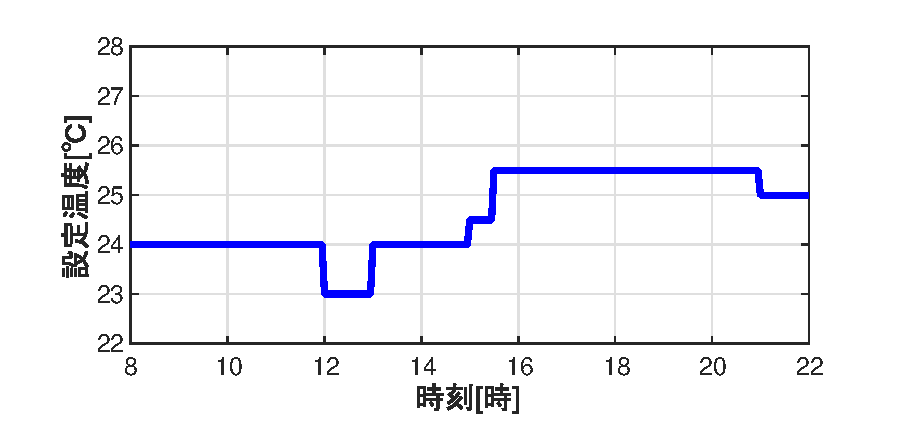
\includegraphics[width=1.0\textwidth,keepaspectratio=true]{fig/math_result_schedule_settemp_j.eps}\\\vspace{0.3cm}{{(j) $|PMV|=0.278$}}
      \end{center}
    \end{minipage}
  \end{center}
  \caption{設定温度パターンの例($\epsilon$=0)}
  \label{fig::math_result_schedule_settemp10}
\end{figure*}

本事例では,探索には\secref{sec::math_setting}で述べた計算環境において,$\epsilon=0$の場合61分3秒,$\epsilon=0.0075$の場合69分50秒, $\epsilon=0.05$の場合75分49秒で計算を終えている.この結果は,直近に配信された正確な気象情報を用いて運転に利用できる,実用的な計算時間であると言える.一方,本章ではビルの一室を対象として最適化を行ったが,ビル全体などさらに大きな規模の環境を対象とする場合は,解評価に必要な数理モデルの計算時間と最適化にかかる時間が増大することが想定される.そのため,対象をビル全体とする場合は計算の高速化が必要である.

\subsection{考察}

(a)パレート解分布\\
探索によって得られたパレート解分布は,制約範囲の境界付近($|$PMV$|\leq 0.1$と$|$PMV$|\geq 0.4$)の解の数が少なかった.これは,数理モデルに原因があると考える.本章で取り扱った数理モデルでは,一日の平均$|$PMV$|$を0もしくは0.5とするには,全ての時間帯でPMV値を0(もしくは-0.5)にしなければならず,設定温度スケジュールも一定値($|$PMV$|\approx0$とするには25.5$^o$C,$|$PMV$|\approx0.5$とするには24$^o$C)にする必要がある.そのため,制約範囲の境界に近いほど設定温度スケジュールが一定値に近くなり変更の余地が少なくなるので,制約範囲の境界付近では多様な解を探索しにくくなり,結果として獲得された解の数が少なかったものと考える.また,$\epsilon$値を大きくすると,制約範囲の境界付近の解が探索できず,解集合の分布も均等でなくなる傾向が見られた.本問題の様に境界付近で探索しにくくなる場合には,$\epsilon$値を大きくして選択圧を上げるよりも,$\epsilon$優越のような優越範囲の変更は行わず,境界付近の解も探索できるようにした方が良いと言える.

(b) 空調設定スケジュール\\
\figref{fig::math_result_schedule}より,平均$|PMV|=0.233$の場合は,各時間帯のPMV値が0に近い場合(16時~22時)と制約値である-0.5に近い場合(8時~14時)があることがわかる.
\figref{fig::math_outside_temp}を見ると,前者は外気温度が比較的高めで,後者は外気温度が低めである.本章で想定する環境条件は冬季であり,空調は暖房動作をしているため,外気温度が高ければ空調のエネルギー消費量は小さくなり,外気温度が低い場合は空調のエネルギー消費量は大きくなる.ここから,PMV値が時間帯によって違う理由は,気温が低くエネルギー消費量が大きくなる時間帯はエネルギー消費量を抑えるためPMV値を-0.5付近に制御し,気温が比較的高くエネルギー消費量が低めの時間帯は快適性を優先しPMV値を0付近に制御していたためであると考えられる.また,\figref{fig::math_result_schedule_settemp10}より,空調の設定温度スケジュールについて,平均$|PMV|=0.233$の様な午後の設定温度を午前よりも高くし昼は設定温度を下げる解以外にも,以下の解のスケジュールがあることがわかる.\\
・昼の時間帯に温度を下げず,午前午後ともに設定温度がほぼ一定であるスケジュール (i)\\
・午前を午後よりも高い設定温度とするスケジュール (b, h)\\
特に制約が無い昼の時間帯に温度を下げないスケジュールがある点や,一日のうち設定温度のピークが異なる時間帯にある解がそれぞれ得られている点から,解のスケジュールには十分な多様性や網羅性がある.そのため,提案手法によって獲得された解集合を候補とすることで,設備管理者は十分豊富な選択肢の中から計画値を決定できると言える.
また,どの解も15:30~17:00の時間は設定温度が25[$^o$C]以上となっている.これは,14時~17時の時間帯は気温が高くエネルギー消費量が低く室内快適性を優先しやすい点と,昼には設定温度を下げるため隣接時間帯との温度差の制約\Eqref{eq::math_constraint_tset_diff}により直後の13時~15時は急激に設定温度を上げられない点によるものと考える.

(c)熱負荷計算方法\\
本章で獲得された空調設定スケジュールでは,予熱運転等をしてもその効果が反映されていない.これは,本章で用いた数理モデルにおける熱負荷計算式が,設定温度・外気温度・室内の発熱のみに依存することを前提としたものであったためと考える.そのため,例えば暖房で温められた部屋の蓄熱量は考慮されずに熱負荷を計算しており,予熱等の効果は反映されなかった.そこで,予熱運転等を考慮した空調設定スケジュールを生成できるよう,熱負荷計算式を改善することや,より正確な熱の推移を計算可能なシミュレータの利用が必要である.

(d)快適性評価モデル\\
本章では,部屋の平均的な温冷感を示す快適性指標PMVを,設定温度と室内機風量設定値を用いた簡易な計算式のみによって計算していた.しかしながら,実際の室温,湿度,風速,平均放射温度は天候や在室者数によっても左右されるため,計算値と不整合が生じる.加えて,在室者の快適性は在室者の座席配置や在室者自身の体調・状況に依存して個人ごとに異なるものであり,PMVは各在室者の快適性を直接表現することができない.そのため,より実際に即した温熱快適性指標と,指標の高速で正確な推定・計算手法を合わせて,目的関数とする必要がある.

\section{ビル管理者の意思決定プロセス}\label{sec::decision_making}
中規模~大規模のオフィスビルの場合,ビル管理者がビルの空調設備を運用している.提案システムでは,室内快適性とエネルギー消費量のトレードオフを示す複数の空調設定温度スケジュールを獲得し,ビル管理者に提示する.ビル管理者は,その中から1つのスケジュールを選択して空調設備運用を行う必要がある.本節では,提案システムで得られた空調設定温度スケジュールの中から,実際に使用するスケジュールを1つ選択する場合の意思決定シナリオを紹介する.
意思決定シナリオの概要を\figref{fig::math_decision_making}に示す.

\begin{figure}[htbp]
  \begin{center}
    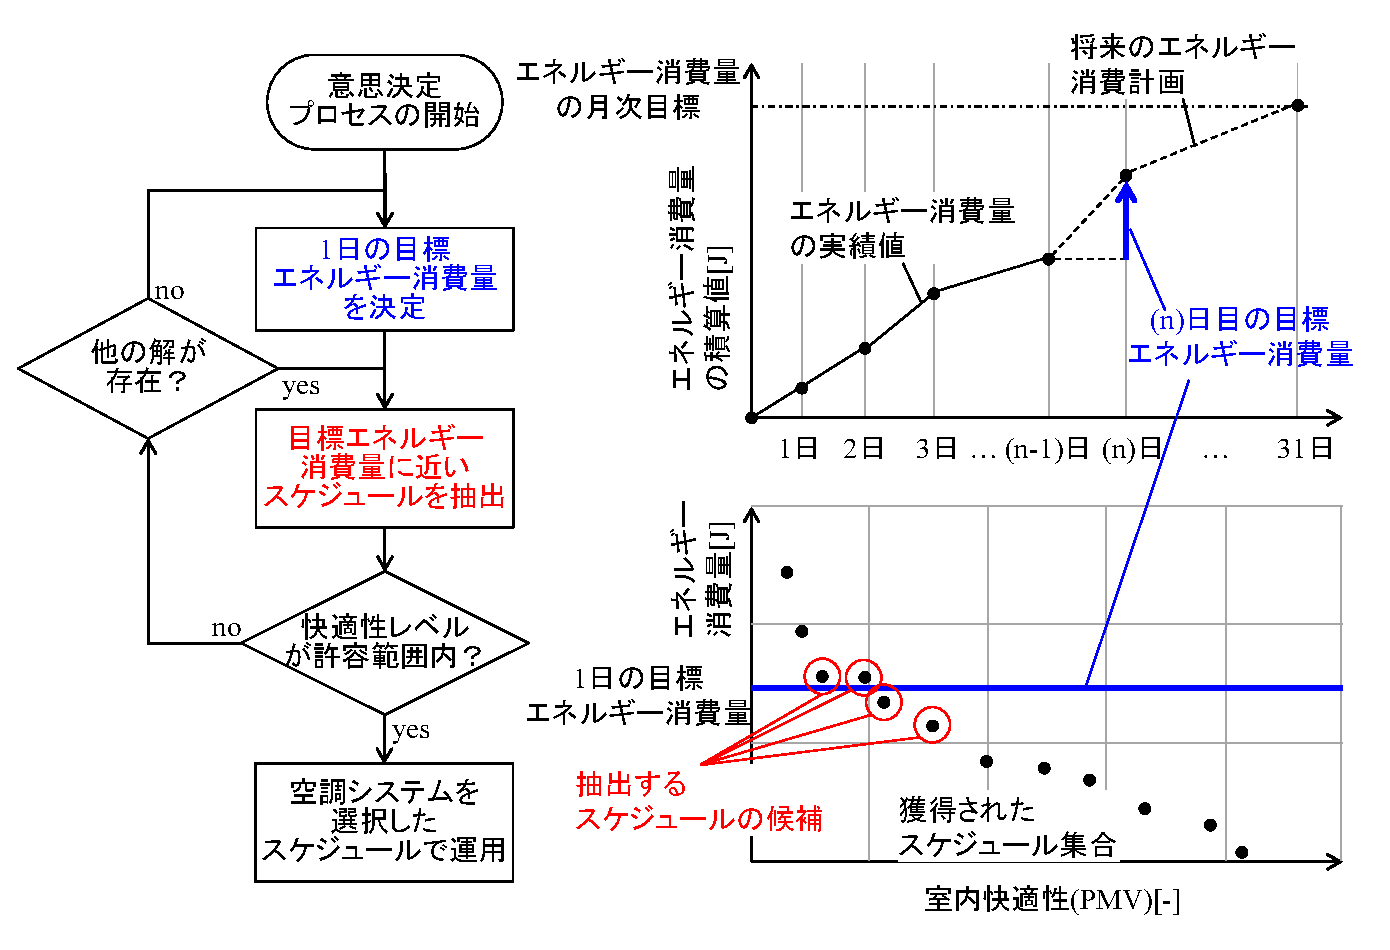
\includegraphics[width=0.8\linewidth]{fig/math_decision_making.eps}
  \end{center}
  \caption{n日目の空調設定スケジュールの意思決定シナリオ}
  \label{fig::math_decision_making}
\end{figure}

まず,ビル管理者は,昨日までの実際のエネルギー消費量と月別のエネルギー消費量の目標値とから,当日のエネルギー消費量の目標値を決定する.その処理を\figref{fig::math_decision_making}の右上に示す.青の実線がその日のエネルギー消費量の目標値を示している.次に,ビル管理者は,目的空間内の最適化されたスケジュールのプロットから,その日の目標エネルギー消費量以下またはそれに近いスケジュールを1つ抽出する.\figref{fig::math_decision_making}の右下に示した赤丸で囲んだスケジュールが,抽出される可能性のあるスケジュールである.すでに目標エネルギー消費量を決定しているので,基本的には目標エネルギー消費量に近いスケジュールを選ぶべきであり,省エネでも快適性が悪いスケジュールを選択する必要はない.その後,ビル管理者は,部屋間の快適性のばらつきをチェックする.許容できるレベルでない場合には,目標エネルギー消費量を中心とした別のスケジュールを選択し,快適性を確認する.目標エネルギー消費量以下のスケジュールがない場合は,その日のエネルギー消費量の目標値を増やして,再度抽出する必要がある.最後に,ビル管理者は,選択された空調設定温度スケジュールで空調システムを運用する.
このように,提案システムは,動的な温度設定スケジュール集合を生成するだけでなく,一日のエネルギー消費量目標値を達成するための意思決定支援も行うことができる.これにより,オフィスワーカーの快適性を維持しつつ,エネルギー消費量の削減に貢献することができる.

\section{結言}
本章では,オフィスの一室の空調設定スケジュールを,数理モデルを用いて最適化する手段について述べた.室内快適性の向上と1日のエネルギー消費量の削減の2つを目的とし,目的関数を数理モデルを用いて定式化した.数理モデルに対してOMOPSOアルゴリズムを適用して,空調設定スケジュールの非劣解集合を探索した.選択圧を変更するパラメータ$\epsilon$を$\epsilon=0$とすることで,エネルギー消費量を削減し快適性を向上できるスケジュールを複数獲得できた.獲得したスケジュール集合は目的関数で広い範囲の解を含んでおり,ビル管理者による意思決定支援が可能であることを示した.

一方で,ビル全体を数理モデル化することに困難がある.本章では,オフィスの一室を数理モデル化したが,数理モデル化の手続きをビル全体に適用する場合,異なる特性を持つ室・熱負荷・設備機器をビルの各部屋に対して設定しなければならない.また,本章では,温湿度,風速等の環境計測値やパラメータの一部に仮定値を用いたが,本来,これらの値は室ごとに空調機と室内の熱移動を考慮して算出する必要がある.そのため,本章の数理モデルをそのままビル全体へ拡張しようとすると,ビルの規模が大きくなるにつれて,正確な数理モデル化が困難になる.

ビル全体の空調最適化のためには,部屋などの相互関係を考慮して室内快適性とエネルギー消費量を正確に評価する手段が必要になる.次章では,ビル全体の室内快適性およびエネルギー消費量を計算・評価する手段としてビルシミュレータを採用し,本章で述べた数理モデルをビルシミュレータによって代替する試みについて述べる.


